\documentclass{article}
\usepackage{graphicx} % Required for inserting images

\title{1NN results- Masters Project}
\author{Maria Ramírez Rodríguez}
\date{February-May 2025}

\begin{document}

\maketitle



\section{Two-dimensional Hubbard model}

The 2D Hubbard model has been an object of scientific study for decades. Theories suggest that this model can accurately resemble the behaviour of cuprate superconductors. In this section a whole phase diagram (as a function of Coulumb repulsion and chemical potential) is studied in detail. 
Functional renormalization group is used to solve (up to a truncated approximation) the Hubbard model hamiltonian for both the nearest neighbour and next nearest neighbour cases.

\subsection{Whole phase diagram}

FRG was used to solve the two-dimensional Hubbard model for several Tight Binding models of varying next-nearest hopping strengths. The calculated points span the whole of the electronic band and include Coulumb repulsion values up to 20eV (or 2.5 times the bandwidth).

- Number of electrons was kept constant by adjusting the chemical potential accordingly

- Displacement of Van Hove singularity- displacement of phase diagram 

- Preservation of stripes- but displacement of them

- SC order parameter

- General trend in SC Tc maximised

- Emergence of CDW phase


\begin{figure}[h] 
    \centering
    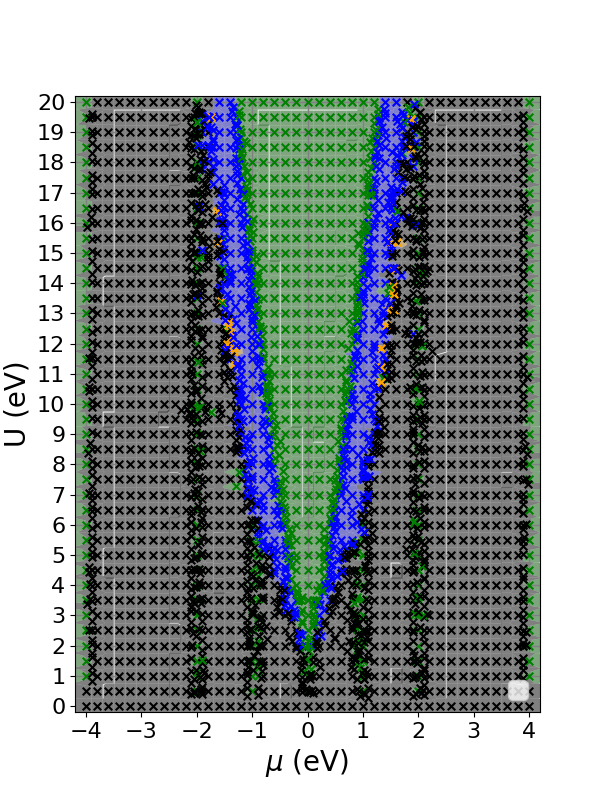
\includegraphics[width=1.20\textwidth]{1NNpd.png} % Change to your image filename
    \caption{An example image}
    \label{fig:Whole phase diagram}
\end{figure}

\subsection{Superconducting region}

After a closer inspection of the superconducting region, one concludes that this phase corresponds to a d-wave superconductor. 
Moreover, the superconducting transition temperature is maximised as the coulomb repulsion increases, closest to the magnetic instability. 



\subsection{Observation of stripes}

- Stripes for integer values of the chemical potential

- Some stripes keep the same magnetic ordering trhoughout

- Others transition from a FM to an AFM

- Stripes displaced with increasing t'



\section{1NNN model}

\subsection{Phase diagrams}

\subsection{Magnetic double dome}

\subsection{Stripes}

\section{La2NiO4}

\subsection{Phase diagram}





\end{document}